La mínima activitat de triti que el detector TRITIUM pot mesurar està limitada per la incertesa del fons radioactiu la qual, com que segueix una estadística de Poisson, depén del nombre d'esdeveniments que es detecten procedents del fons radioactiu. Per tant, per reduir en la mesura del possible la mínima activitat de triti mesurable, s'ha de minimitzar tant com siga possible els esdeveniments detectats procedents del fons radioactiu. El fons radioactiu que és mesurat pel detector TRITIUM procedeix de dues fonts principals, els elements radioactius presents al medi ambient (principalment $\ce{^{40}K}$ i $\ce{^{226}Ra}$) i la radiació còsmica.

Per a reduir el nombre d'esdeveniments del fons radioactiu detectats pel detector TRITIUM s'ha dissenyat i construït un sistema de rebuig del fons radioactiu que consisteix en dues parts:

\begin{enumerate}

\item{} Un castell de plom amb parets de $5~\cm$ de gruix, mostrat a la Figura \ref{subfig:CastellPlom}, a l'interior del qual se situa el detector. Aquest frena les partícules de menor energia (fins a $200~\MeV$), les quals procedeixen principalment de les partícules radioactives del medi ambient i part dels rajos còsmics.

\item{} Un veto actiu, que consisteix en dos blocs de plàstic centellejador, amb un espectre d'emissió mostrat a la Figura \ref{subfig:EspectreEmisioVeto}, els quals són llegits per PMTs model R$8520-406$ de Hamamatsu Photonics. Aquests plàstics estan envoltats amb capes de PTFE, alumini i cinta negra per a millorar la col·lecció dels fotons generats i la uniformitat del senyal, millora quantificada experimentalment amb un factor dos.
\begin{figure}
\centering
    \begin{subfigure}[b]{0.7\textwidth}
    \centering
    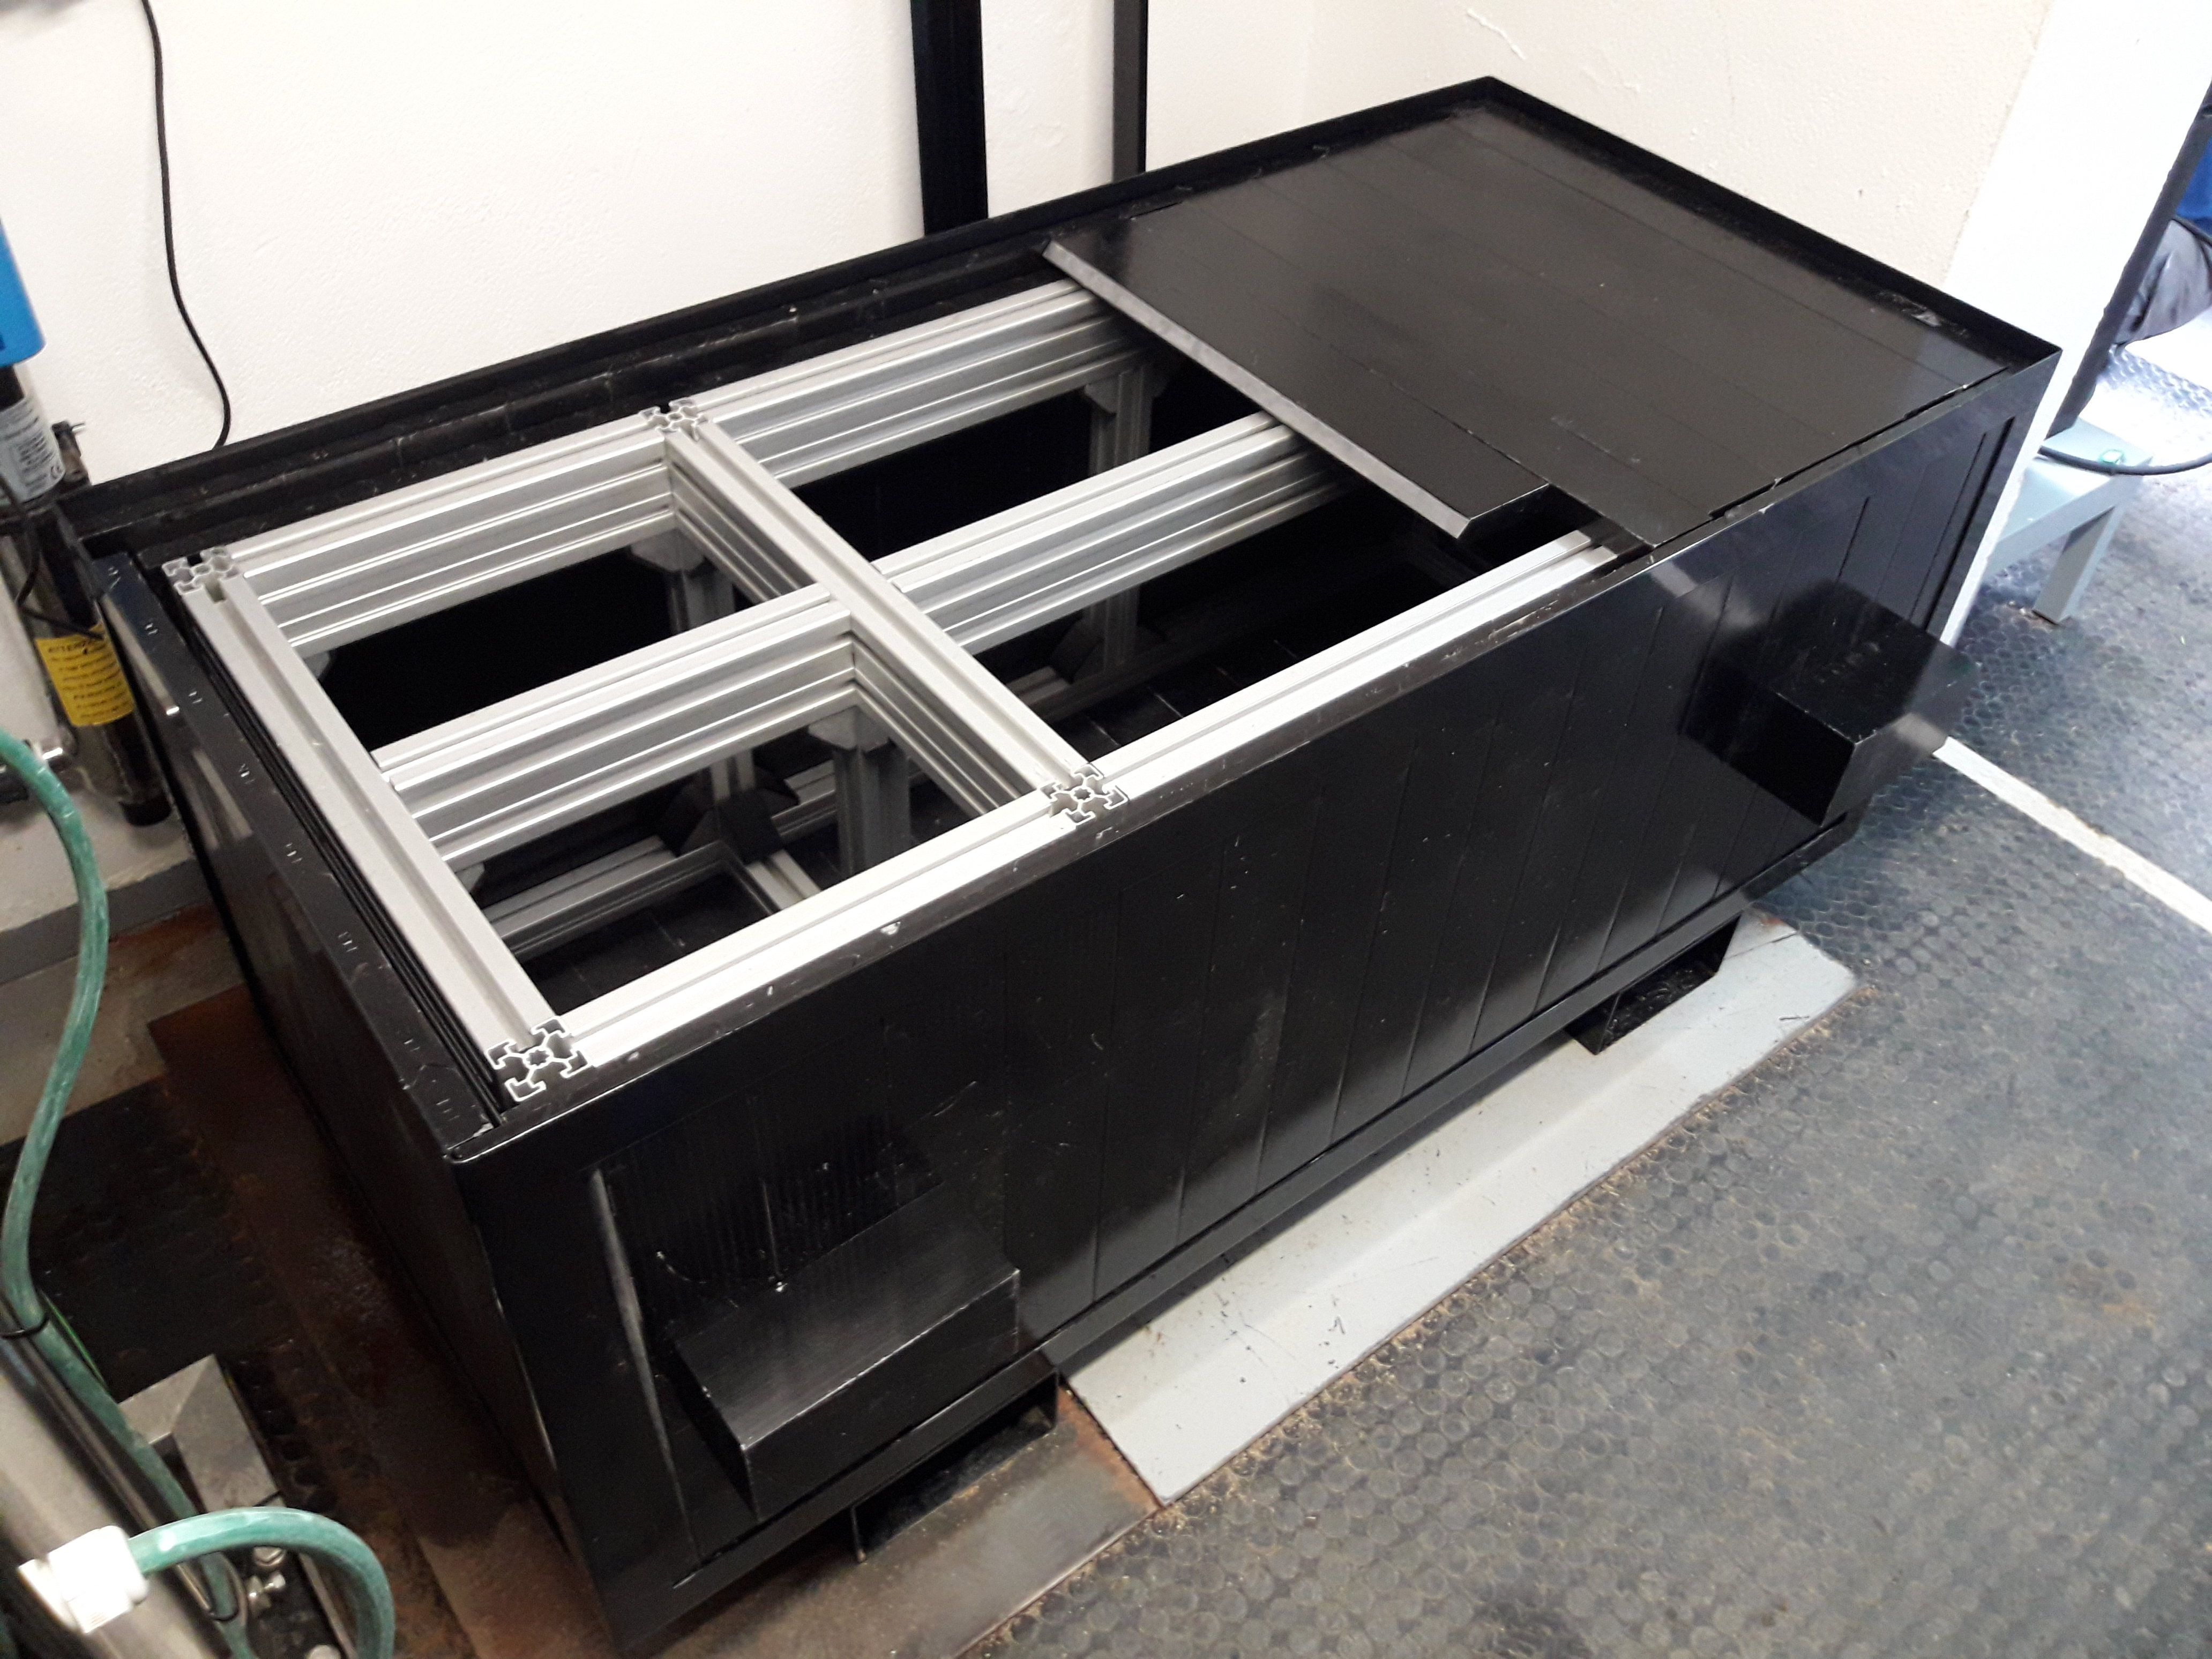
\includegraphics[width=\textwidth]{12Summary/3DesignPrinciples/34BackgroundRejectionSystem/AluminiumStructure.jpg}  
        \caption{}\label{subfig:CastellPlom}
    \end{subfigure}
    \hfill
    \begin{subfigure}[b]{0.7\textwidth}
    \centering
    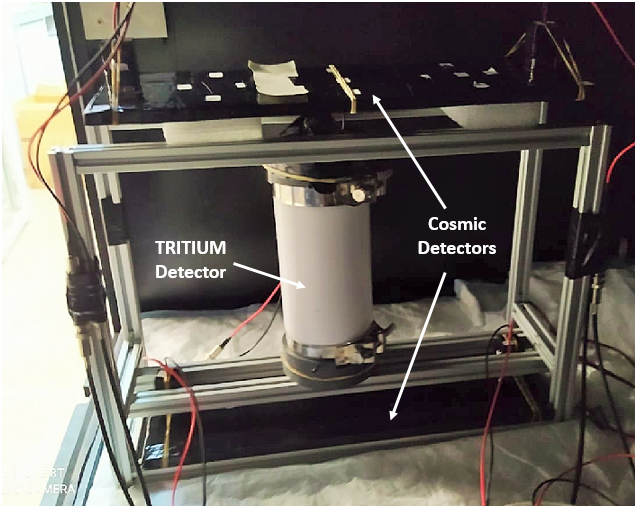
\includegraphics[width=\textwidth]{12Summary/3DesignPrinciples/34BackgroundRejectionSystem/Vetos_y_prototipo.png}  
    \caption{\label{subfig:VetoActiu}}
    \end{subfigure}
\caption{Parts del sistema de rebuig del fons radioactiu dissenyat per la col·laboració TRITIUM: a) Castell de plom. b) Veto actiu. \label{fig:SistemaRebuigFonsRadioactiu}}
\end{figure}
Aquests estan situats a l'interior del castell de plom, un dalt i l'altre baix del detector de triti, com es pot veure a la imatge \ref{subfig:VetoActiu}. Els plàstics centellejadors són llegits en anticoincidència amb el detector de triti per a eliminar els esdeveniments del fons que aconsegueixen travessar el castell de plom, principalment rajos còsmics amb energies superiors al $200~\MeV$. 

Es va mesurar l'espectre d'energia de rajos còsmics durs (energies superiors a $200~\MeV$), el qual es mostra a la Figura \ref{fig:EspectreEnergeticVetoActiu}. Aquest espectre es va utilitzar per a determinar la freqüència de rajos còsmics mesurats, $2,5~\text{events}/\sec$, la qual, comparant amb l'esperat per a un veto actiu d'aquestes dimensions al nivell del mar, va permetre obtenir una eficiència de detecció als rajos còsmics d'alta energia d'al voltant d'un $85\%$.

\begin{figure}[h]
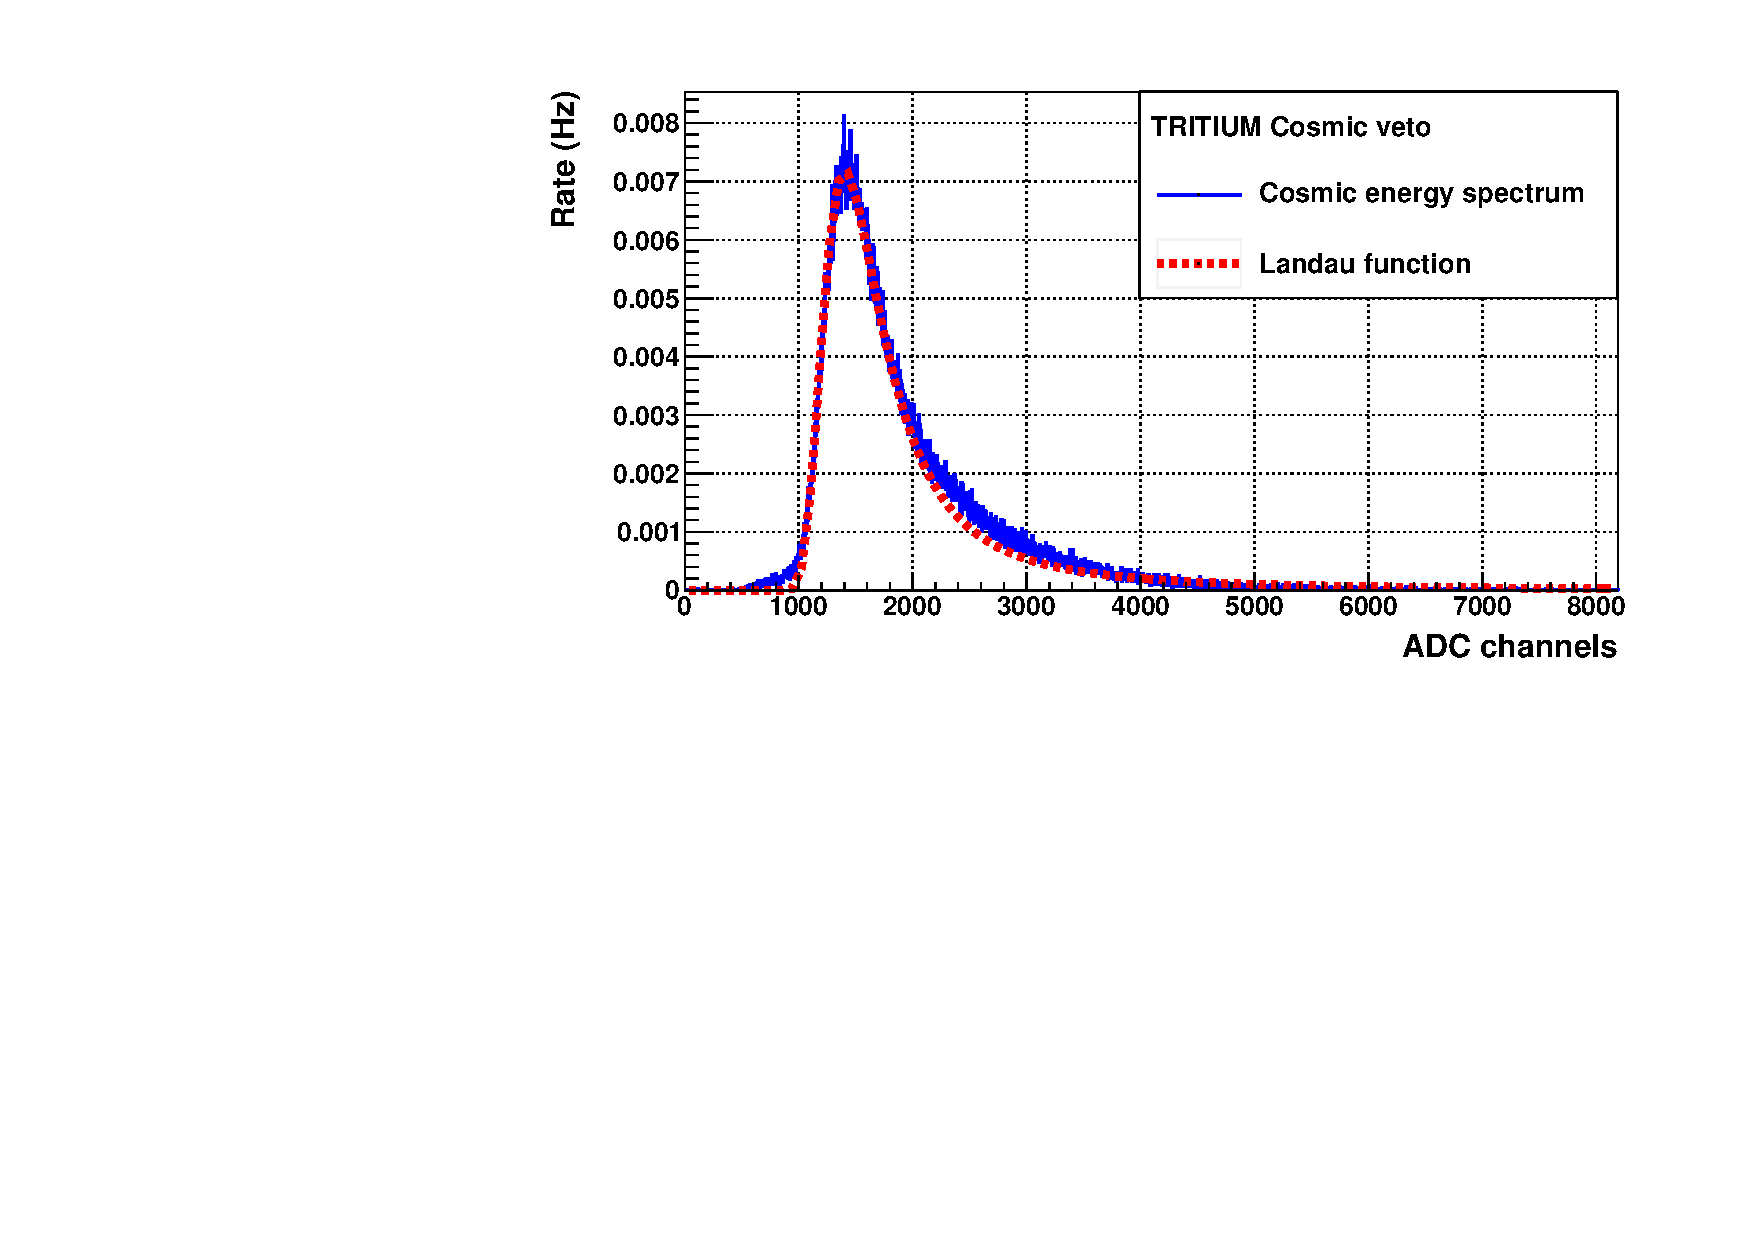
\includegraphics[scale=0.7]{12Summary/4ResearchAndDevelopments/43CosmicVetos/Cosmic_Energy_Spectrum_36_cm_Landau_Function.pdf}
\centering
\caption{Espectre d'energia dels rajos còsmics d'alta energia (energies superiors a $200~\MeV$) mesurat amb el veto actiu desenvolupat a la col·laboració TRITIUM\label{fig:EspectreEnergeticVetoActiu}.}
\end{figure}

\end{enumerate} 